\subsection{Dataset 1 (Univariate)}
\begin{flushleft}
Here, we are required to do curve fitting of the function $e^{cos(2 \pi x)}$. For this purpose we use a training set of 1000 points.



\end{flushleft}


\begin{flushleft}

\textbf{MLFFNN :}
For the uni-variate dataset, we use a feed-forward network with 1 hidden layer. The number of nodes in the hidden layer represents the model complexity, which is estimated by looking at the performance on the validation dataset. We varies the number of hidden layer nodes from 1 to 200, and compared the performance   (MSE) on all the three sets. The plot showing the variation of MSE w.r.t model complexity is shown below :

\end{flushleft}


\begin{figure}[H]
\centering
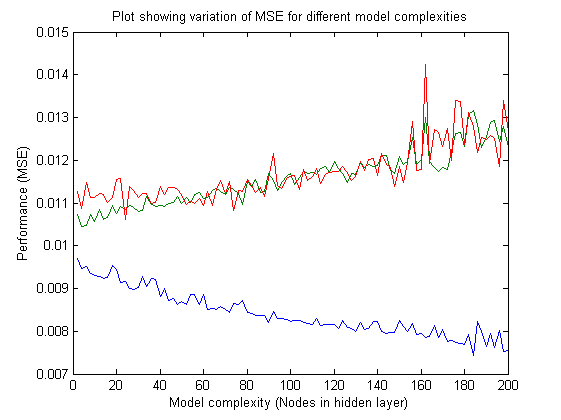
\includegraphics[width=\linewidth]{Regression/univariate/mse.png}
\caption{Legend: Blue-Train  Green-Validation R-Test}
\end{figure}

From the above plot, we can see that the train error decreases on increasing the model complexity. This is expected, as a high number of nodes in the hidden layer leads to overfitting of the training data. So, the best neural network configuration is chosen as the one which gives least MSE on the validation data.
The configuration obtained is shown below, with 4 nodes in the hidden layer.


\begin{figure}[H]
\centering
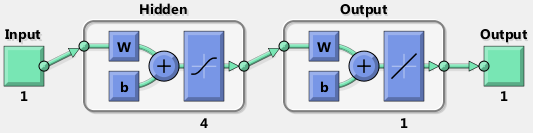
\includegraphics[width=0.6\linewidth]{Regression/univariate/net_config.png}
\caption{Neural network configuration}
\end{figure}

For this configuration, the plots of model and target outputs are shown in the figures below : 

\begin{figure}[H]
\centering
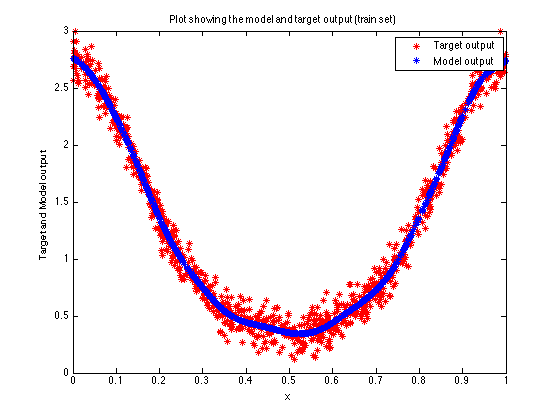
\includegraphics[width=0.5\linewidth]{Regression/univariate/trainOutput.png}
\caption{Plots of model and target output (Train data)}
\end{figure}

\begin{figure}[H]
\centering
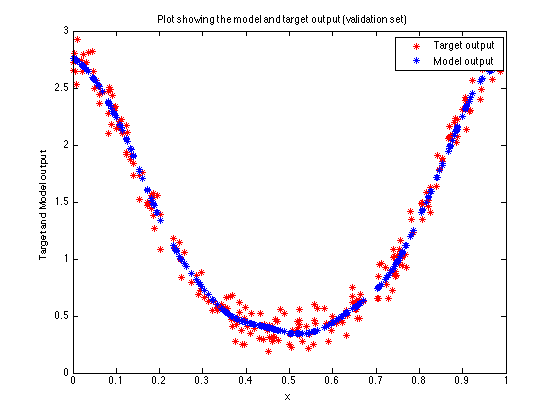
\includegraphics[width=0.5\linewidth]{Regression/univariate/valOutput.png}
\caption{Plots of model and target output (Validation data)}
\end{figure}

\begin{figure}[H]
\centering
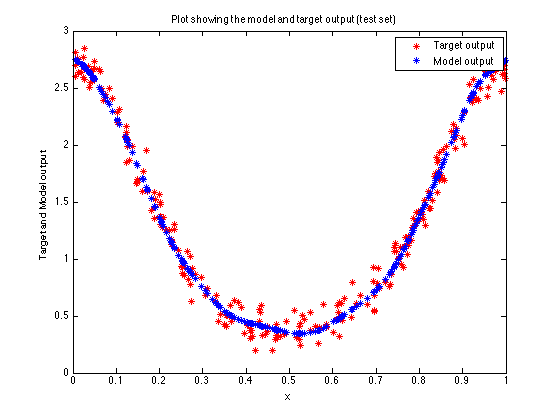
\includegraphics[width=0.5\linewidth]{Regression/univariate/testOutput.png}
\caption{Plots of model and target output (Test data)}
\end{figure}

\begin{flushleft}
From the plots, we can see that the model output closely follows the target output in all of the three plots, which shows the generalization ability of the neural network model.

Scatter plot with target output on $x$-axis and model output on $y$-axis for train, validation, test data is as follows:

\end{flushleft}

\begin{figure}[H]
\centering
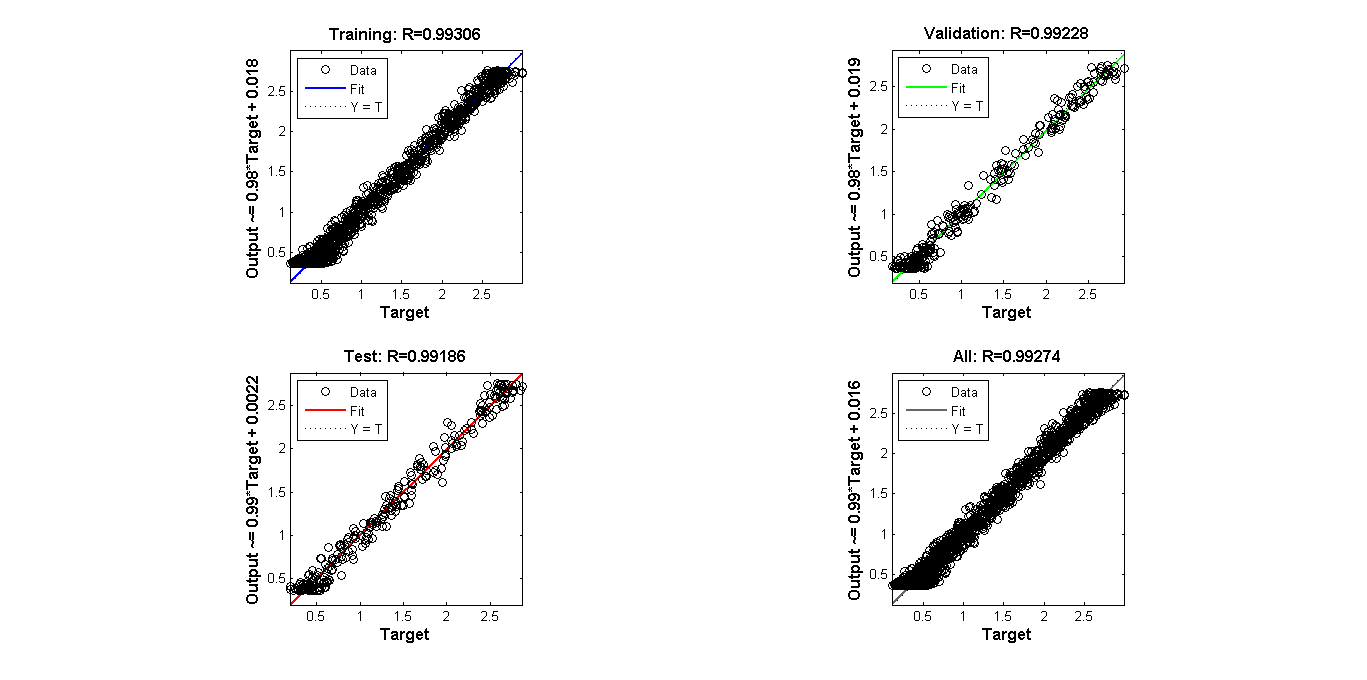
\includegraphics[width=1.2\linewidth]{Regression/univariate/Scatter_plots.png}
\caption{Scatter plots of model and target output}
\end{figure}


\begin{flushleft}
Again from the scatter plots shown above, we can validate the correctness of the model obtained by observing that the scatter plot follows the $y = x$ line closely. 
\end{flushleft}
\newpage

\textbf{Output of output node after different number of epochs:}

\begin{figure}[H]
\centering
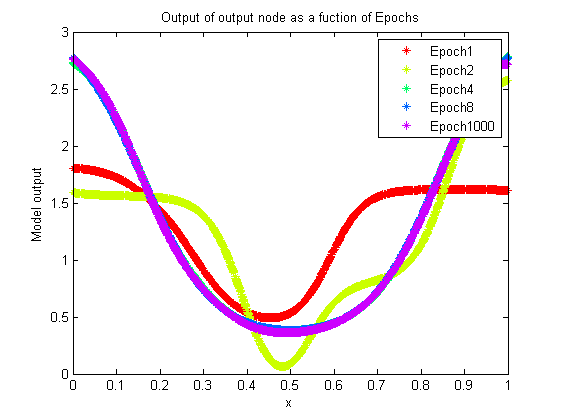
\includegraphics[width=0.6\linewidth]{Regression/univariate/epoch_output.png}
\caption{Output of output nodes for different epochs}
\end{figure}

\begin{flushleft}

Here, we see that the neural network model starts with bad fit to the training data, and the model output progressively becomes closer to the true function (curve), as the number of epochs increase. The epoch number 1000 just represents the end of training phase. This is also expected as the neural network's performance improves over the epochs till the error function's value becomes nearly zero. 
\end{flushleft}

\newpage
\textbf{Output of hidden layer nodes for different number of epochs: \\[10pt]}

\begin{figure}
\begin{subfigure}{.5\textwidth}
  \centering
  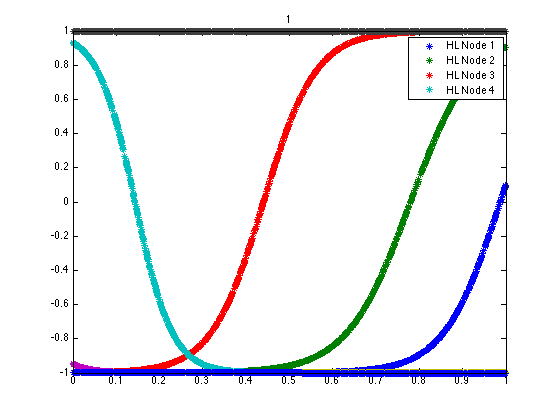
\includegraphics[width=.8\linewidth]{Regression/univariate/hiddenLayer_1.png}\
  \caption{Epoch 1}
\end{subfigure}%
\begin{subfigure}{.5\textwidth}
  \centering
  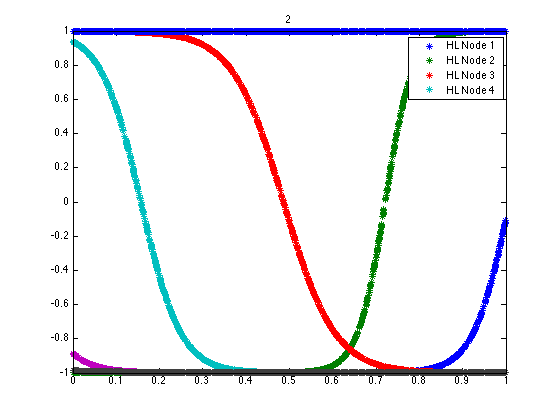
\includegraphics[width=.8\linewidth]{Regression/univariate/hiddenLayer_2.png}
   \caption{Epoch 2}
  \end{subfigure}
  \begin{subfigure}{.5\textwidth}
  \centering
  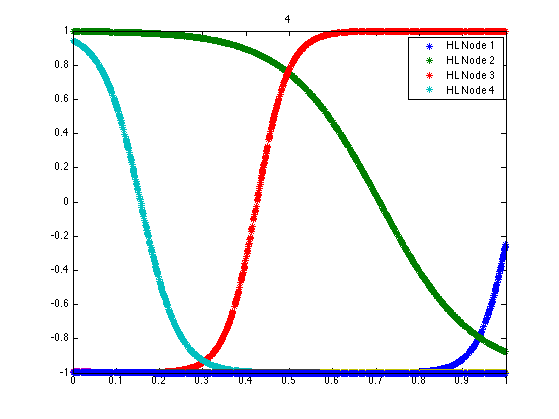
\includegraphics[width=.8\linewidth]{Regression/univariate/hiddenLayer_4.png}\
  \caption{Epoch 4}
\end{subfigure}%
\begin{subfigure}{.5\textwidth}
  \centering
  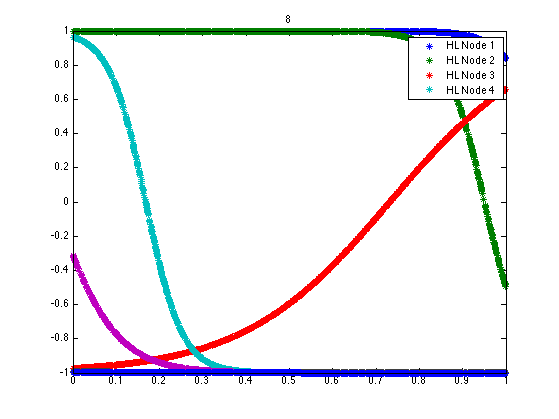
\includegraphics[width=.8\linewidth]{Regression/univariate/hiddenLayer_8.png}
   \caption{Epoch 8}
  \end{subfigure}
  
  \begin{subfigure}{0.5\textwidth}
  \centering
  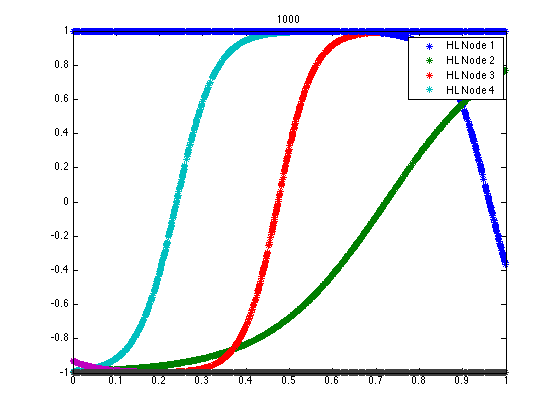
\includegraphics[width=0.8\linewidth]{Regression/univariate/hiddenLayer_1000.png}
   \caption{End of training}
  \end{subfigure}
  
\caption{Output of hidden layer nodes}
\end{figure}


\textbf{Observations :}

\begin{itemize}
\item In general, it was observed that neural network model was decently accurate in the fitting of a non-linear curve. 
\item The model output closely followed the target output in general. 
\item The values of MSE on train, val and test obtained for the best model were 0.0096, 0.0106 and 0.0112. \item These indicate that the model not only fits the train data properly, but also generalizes very well.
\end{itemize}



\subsection{Dataset 2 (Bivariate)}

\textbf{MLFFNN with 1 hidden layer:}

\begin{flushleft}
For the bi-variate dataset, we first use a feed-forward network with 1 hidden layer. The number of nodes in the hidden layer represents the model complexity, which is estimated by looking at the performance on the validation dataset. We varies the number of hidden layer nodes from 1 to 200, and compared the performance (MSE) on all the three sets. The plot showing the variation of MSE w.r.t model complexity is shown below :

\end{flushleft}


\begin{figure}[H]
\centering
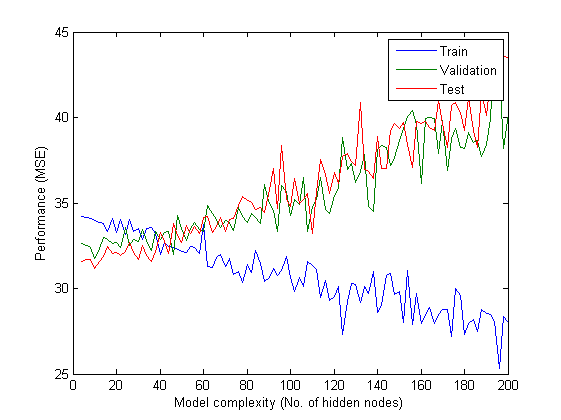
\includegraphics[width=0.8\linewidth]{Regression/bivariate/1layer_mse.png}
\caption{MSE vs Model Complexity}
\end{figure}

Here again, we observe similar trends as the previous case and the best configuration is obtained by choosing the model that gives the best validation performance.
The best neural network configuration obtained is shown below, with 8 nodes in the hidden layer.

\begin{figure}[H]
\centering
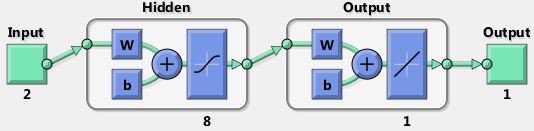
\includegraphics[width=0.6\linewidth]{Regression/bivariate/net_config.png}
\caption{Neural network configuration}
\end{figure}

For this configuration, the plots of model and target outputs are shown in the figures below : 

\begin{figure}[H]
\centering
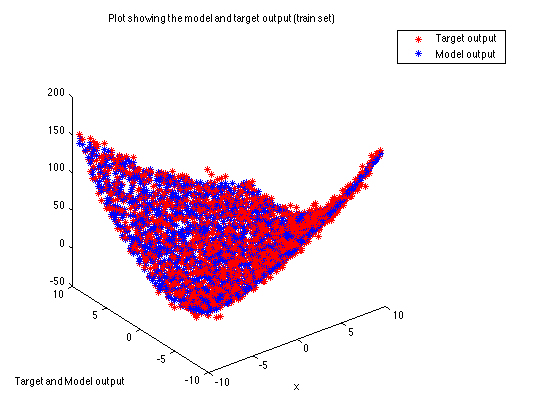
\includegraphics[width=0.5\linewidth]{Regression/bivariate/output_1layer_train.png}
\caption{Plots of model and target output (Train data)}
\end{figure}

\begin{figure}[H]
\centering
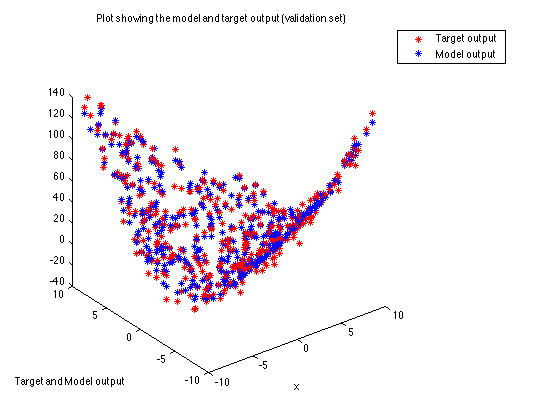
\includegraphics[width=0.5\linewidth]{Regression/bivariate/output_1layer_val.png}
\caption{Plots of model and target output (Validation data)}
\end{figure}

\begin{figure}[H]
\centering
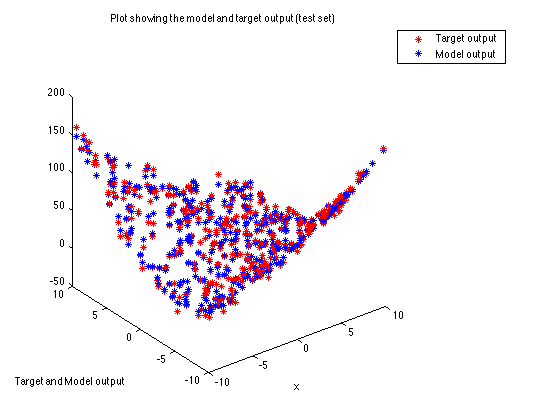
\includegraphics[width=0.5\linewidth]{Regression/bivariate/output_1layer_test.png}
\caption{Plots of model and target output (Test data)}
\end{figure}

\begin{flushleft}
In this dataset, the true surface is bowl shaped.  We can see that in all of the three plots, the model output also closely resembles this surface and closely follows the target output also. This can be verified by looking the scatter plots obtained below :
\end{flushleft}

Scatter plot with target output on $x$-axis and model output on $y$-axis for train, validation, test data is as follows:

\begin{figure}[H]
\centering
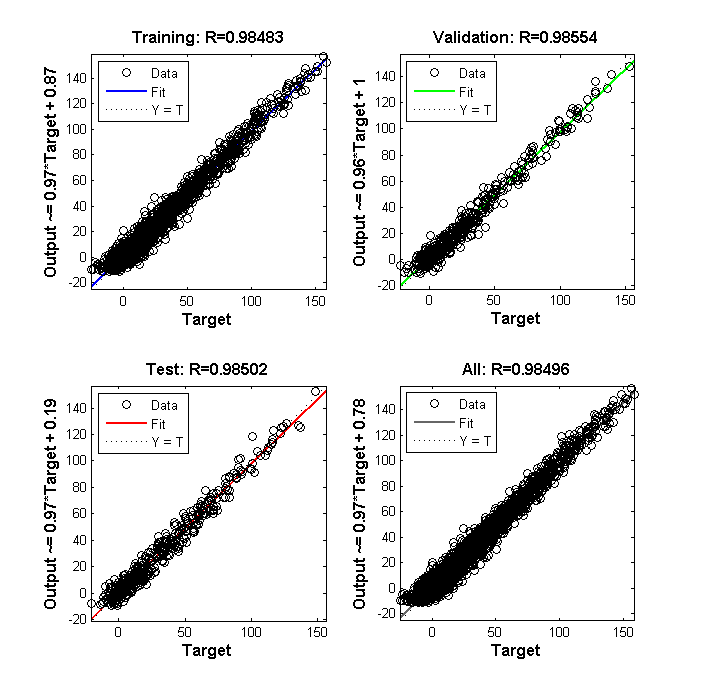
\includegraphics[width=\linewidth]{Regression/bivariate/scatter_1layer.png}
\caption{Scatter plots of model and target output}
\end{figure}

Here, in the scatter plots obtained we observe a $y = x$ for both train and validation datasets. But, for the test data, the best fit line deviates slightly from the $y = x$ line. This is because of slight overfitting which is present, even though the model with the complexity is chosen based on validation. 


\textbf{Output of output node after different number of epochs: } \\[10pt] 

\begin{figure}
\begin{subfigure}{.5\textwidth}
  \centering
  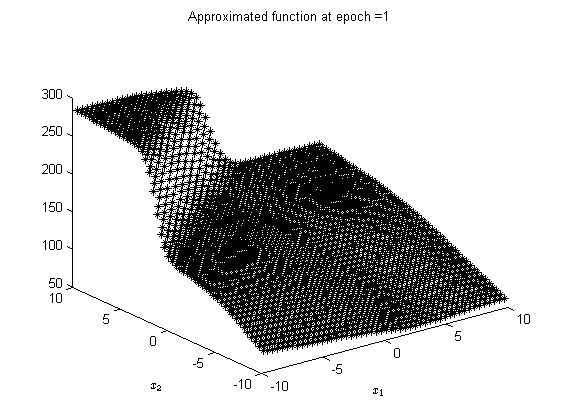
\includegraphics[width=.8\linewidth]{Regression/bivariate/1layer_epoch_1.png}\
  \caption{Epoch 1}
\end{subfigure}%
\begin{subfigure}{.5\textwidth}
  \centering
  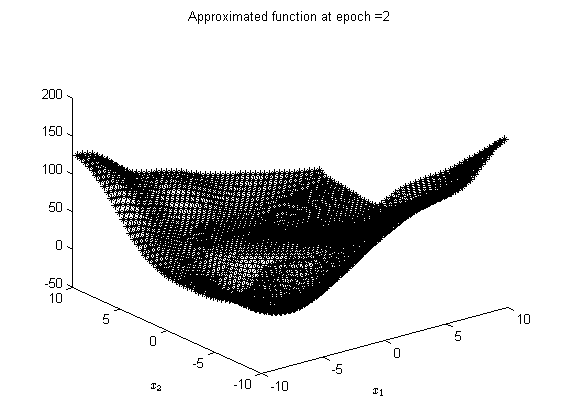
\includegraphics[width=.8\linewidth]{Regression/bivariate/1layer_epoch_2.png}
   \caption{Epoch 2}
  \end{subfigure}
  
  \begin{subfigure}{.5\textwidth}
  \centering
  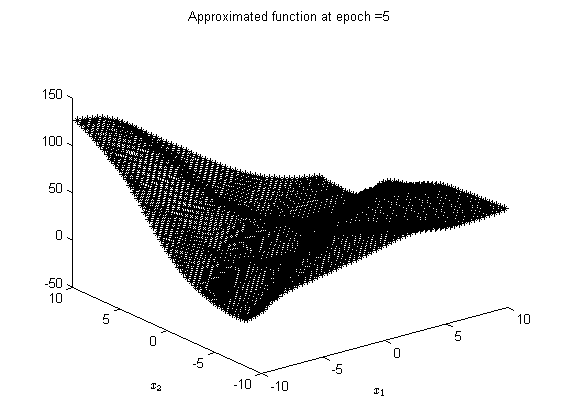
\includegraphics[width=.8\linewidth]{Regression/bivariate/1layer_epoch_5.png}\
  \caption{Epoch 5}
\end{subfigure}%
\begin{subfigure}{.5\textwidth}
  \centering
  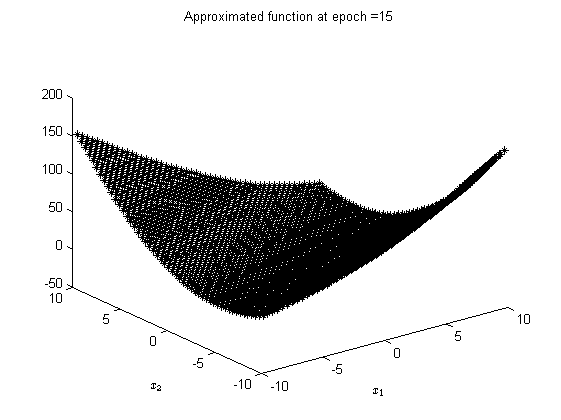
\includegraphics[width=.8\linewidth]{Regression/bivariate/1layer_epoch_15.png}
   \caption{Epoch 15}
  \end{subfigure}
  
  \begin{subfigure}{.5\textwidth}
  \centering
  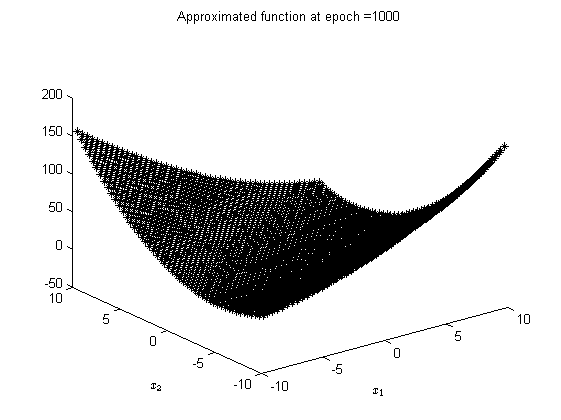
\includegraphics[width=.8\linewidth]{Regression/bivariate/1layer_epoch_1000.png}\
  \caption{End of training}
\end{subfigure}%
  
\caption{Output of output layer node}
\end{figure}

\newpage

\textbf{Output of hidden layer node (one of the nodes) after different number of epochs:}

\begin{figure}
\begin{subfigure}{.5\textwidth}
  \centering
  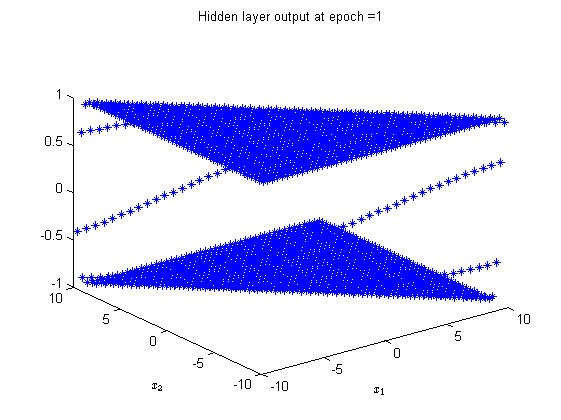
\includegraphics[width=.8\linewidth]{Regression/bivariate/hidden_1layer_1.png}\
  \caption{Epoch 1}
\end{subfigure}%
\begin{subfigure}{.5\textwidth}
  \centering
  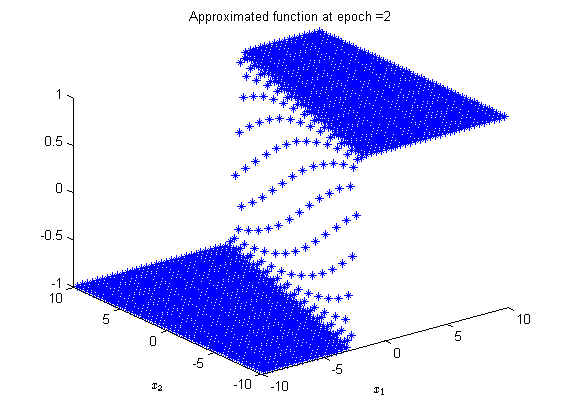
\includegraphics[width=.8\linewidth]{Regression/bivariate/hidden_1layer_2.png}
   \caption{Epoch 2}
  \end{subfigure}
  
  \begin{subfigure}{.5\textwidth}
  \centering
  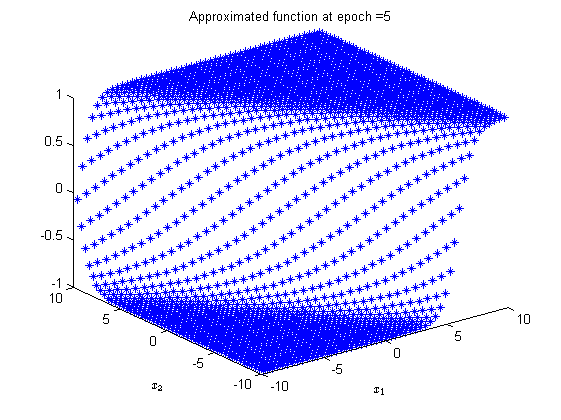
\includegraphics[width=.8\linewidth]{Regression/bivariate/hidden_1layer_5.png}\
  \caption{Epoch 5}
\end{subfigure}%
\begin{subfigure}{.5\textwidth}
  \centering
  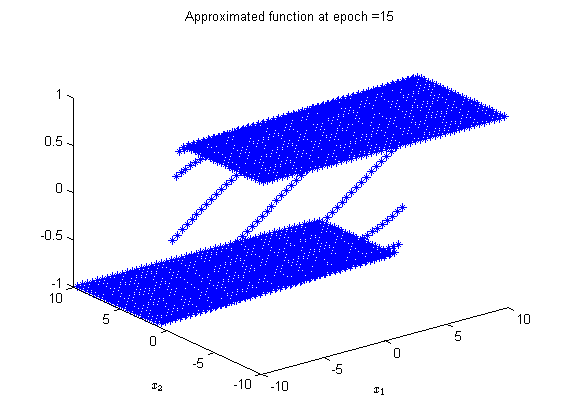
\includegraphics[width=.8\linewidth]{Regression/bivariate/hidden_1layer_15.png}
   \caption{Epoch 15}
  \end{subfigure}
  
  \begin{subfigure}{.5\textwidth}
  \centering
  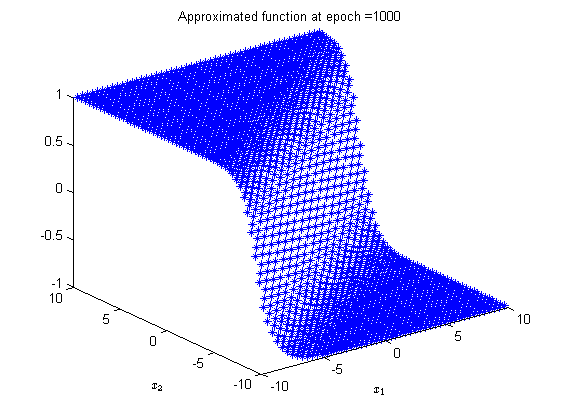
\includegraphics[width=.8\linewidth]{Regression/bivariate/hidden_1layer_1000.png}\
  \caption{End of training}
\end{subfigure}%
  
\caption{Output of hidden layer node}
\end{figure}










\textbf{MLFFNN with 2 hidden layers:}

For the bi-variate dataset, we first use a feed-forward network with 2 hidden layers. The number of nodes in each hidden layer represents the model complexity, which is estimated by looking at the performance on the validation dataset. We varies the number of hidden layer nodes from 1 to 200 (ensuring that the second layer has lesser nodes than the first), and compared the performance (MSE) on all the three sets. 

The best neural network configuration obtained is shown below, with 15 nodes in the first hidden layer and 10 in the second hidden layer.

\begin{figure}[H]
\centering
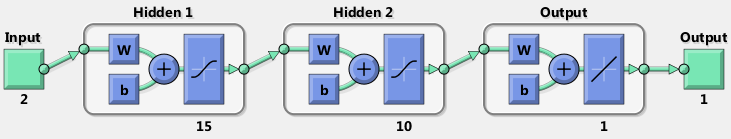
\includegraphics[width=\linewidth]{Regression/bivariate/net_config_2.png}
\caption{Neural network configuration}
\end{figure}

For this configuration, the plots of model and target outputs are shown in the figures below : 

\begin{figure}[H]
\centering
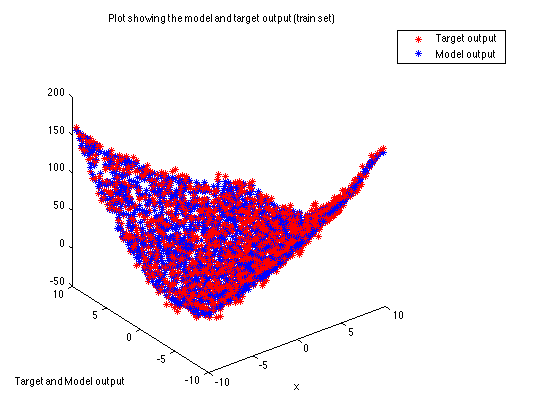
\includegraphics[width=0.5\linewidth]{Regression/bivariate/output_2layer_train.png}
\caption{Plots of model and target output (Train data)}
\end{figure}

\begin{figure}[H]
\centering
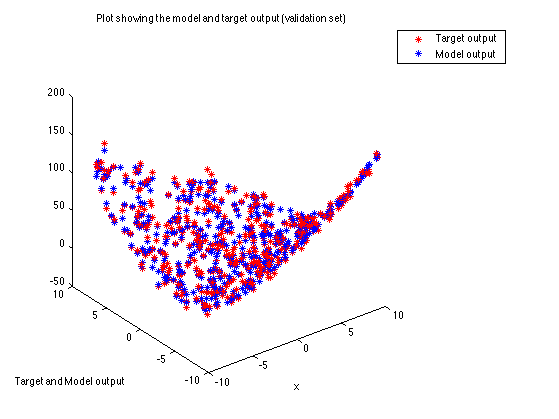
\includegraphics[width=0.5\linewidth]{Regression/bivariate/output_2layer_val.png}
\caption{Plots of model and target output (Validation data)}
\end{figure}

\begin{figure}[H]
\centering
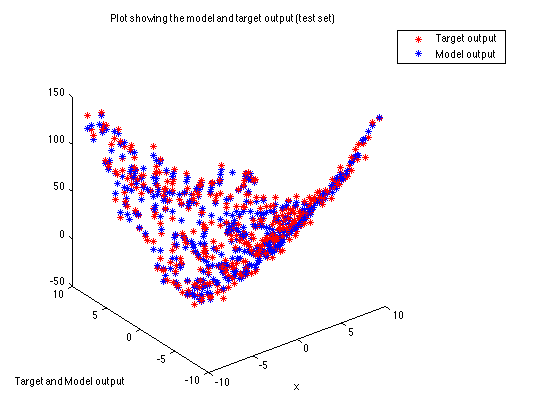
\includegraphics[width=0.5\linewidth]{Regression/bivariate/output_2layer_test.png}
\caption{Plots of model and target output (Test data)}
\end{figure}

\begin{flushleft}

Here again, as in the earlier case the model outputs closely resemble the true surface of data to be fut, which is bowl shaped.
Scatter plot with target output on $x$-axis and model output on $y$-axis for train, validation, test data is as follows:
\end{flushleft}


\begin{figure}[H]
\centering
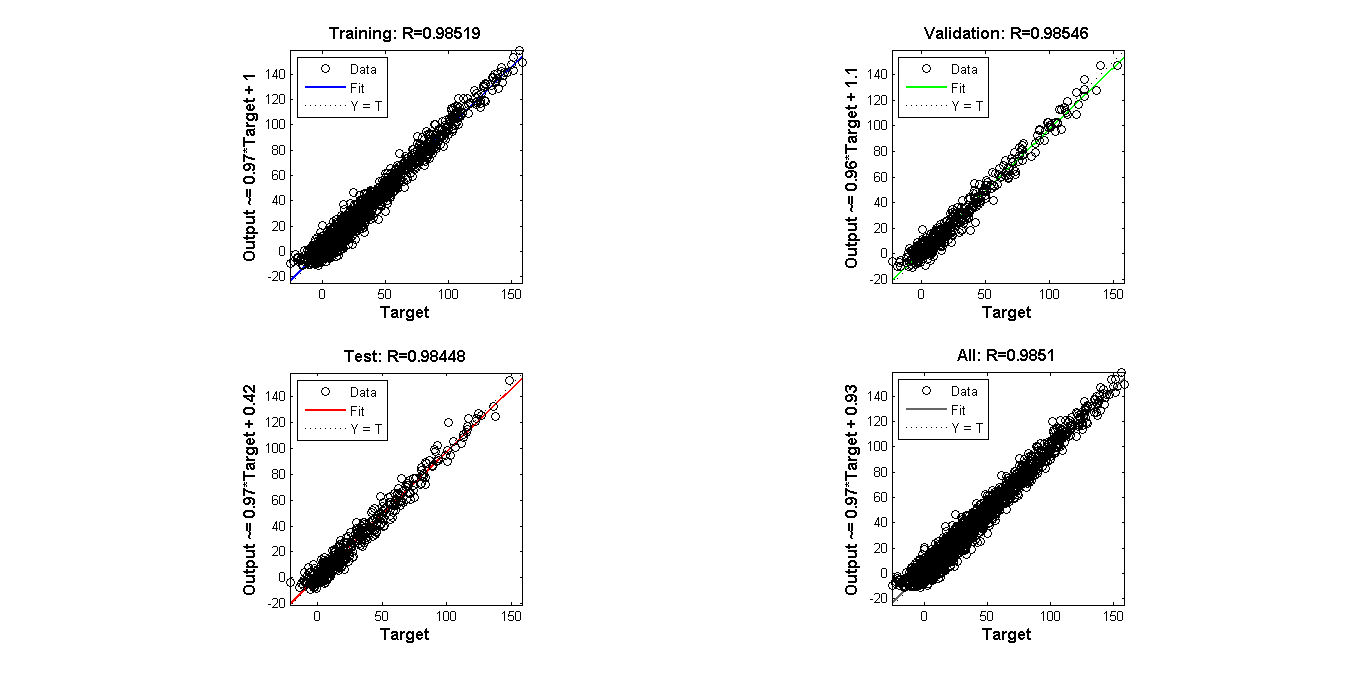
\includegraphics[width=1.2\linewidth]{Regression/bivariate/scatter_2layers.png}
\caption{Scatter plots of model and target output}
\end{figure}

Here, we observe very slight deviations from the $y = x$ line for the test and validation scatter plots. This is because of the slight overfitting caused by using 2 layers in the neural network.
The plot of output of output node after different number of epochs:

\begin{figure}
\begin{subfigure}{.5\textwidth}
  \centering
  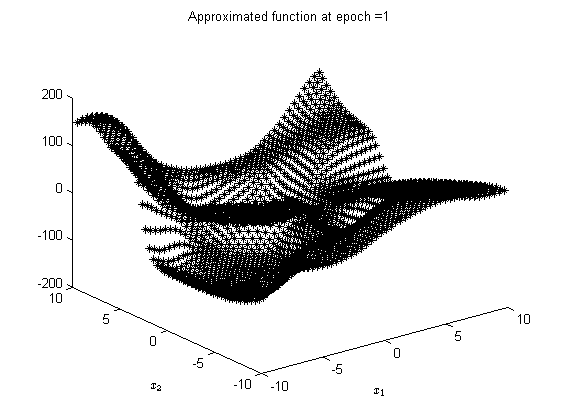
\includegraphics[width=.8\linewidth]{Regression/bivariate/2layers_epoch_1.png}\
  \caption{Epoch 1}
\end{subfigure}%
\begin{subfigure}{.5\textwidth}
  \centering
  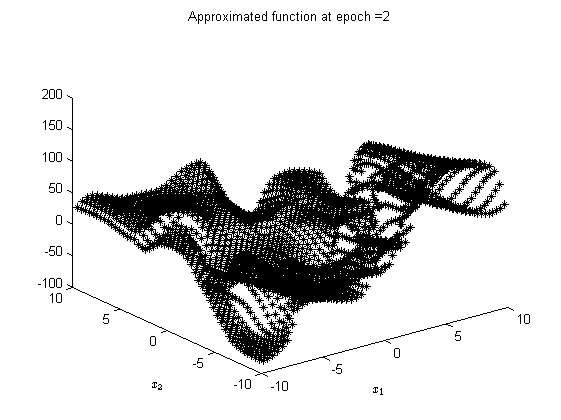
\includegraphics[width=.8\linewidth]{Regression/bivariate/2layers_epoch_2.png}
   \caption{Epoch 2}
  \end{subfigure}
  
  \begin{subfigure}{.5\textwidth}
  \centering
  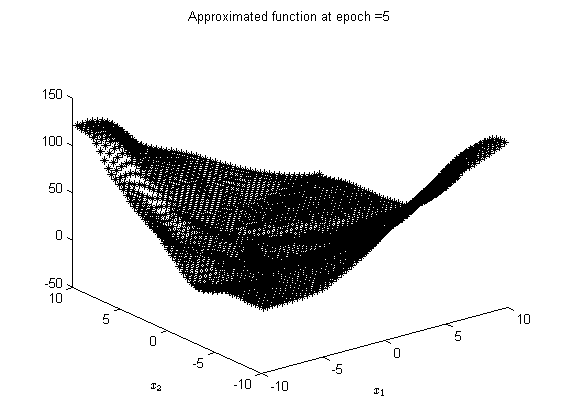
\includegraphics[width=.8\linewidth]{Regression/bivariate/2layers_epoch_5.png}\
  \caption{Epoch 5}
\end{subfigure}%
\begin{subfigure}{.5\textwidth}
  \centering
  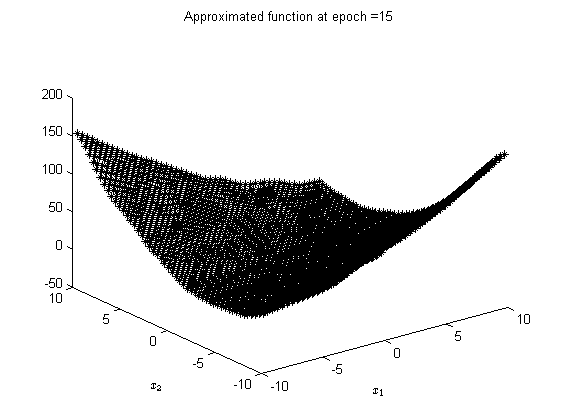
\includegraphics[width=.8\linewidth]{Regression/bivariate/2layers_epoch_15.png}
   \caption{Epoch 15}
  \end{subfigure}
  
  \begin{subfigure}{.5\textwidth}
  \centering
  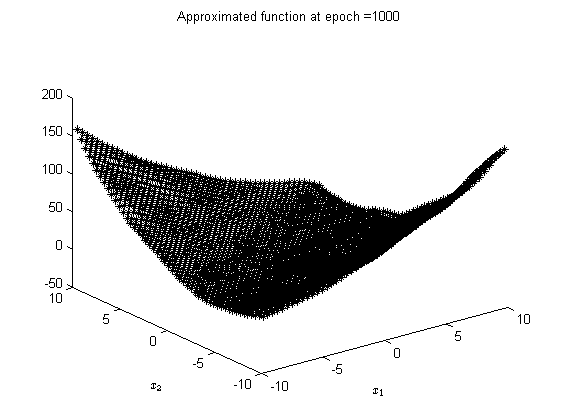
\includegraphics[width=.8\linewidth]{Regression/bivariate/2layers_epoch_1000.png}\
  \caption{End of training}
\end{subfigure}%
  
\caption{Output of output layer node}
\end{figure}

The plot of output of hidden layer 1 node (one of the nodes) after different number of epochs:

\begin{figure}
\begin{subfigure}{.5\textwidth}
  \centering
  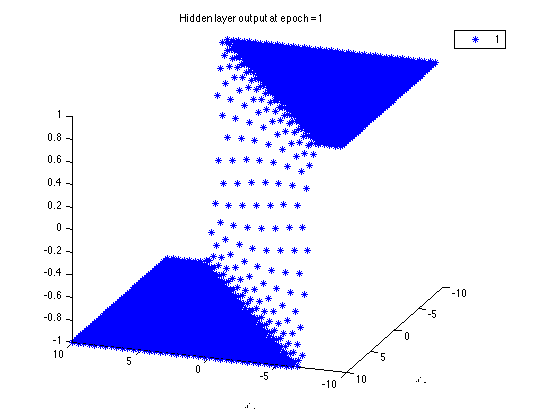
\includegraphics[width=.8\linewidth]{Regression/bivariate/hidden_2layer_1.png}\
  \caption{Epoch 1}
\end{subfigure}%
\begin{subfigure}{.5\textwidth}
  \centering
  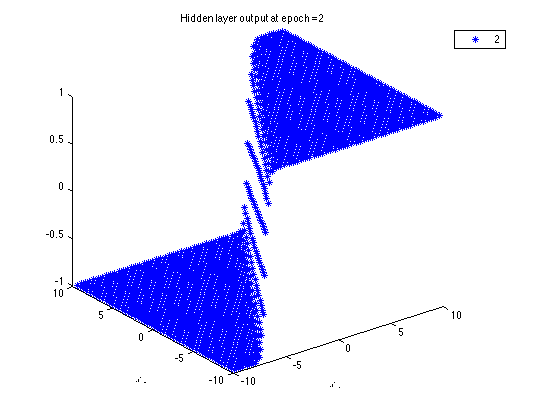
\includegraphics[width=.8\linewidth]{Regression/bivariate/hidden_2layer_2.png}
   \caption{Epoch 2}
  \end{subfigure}
  
  \begin{subfigure}{.5\textwidth}
  \centering
  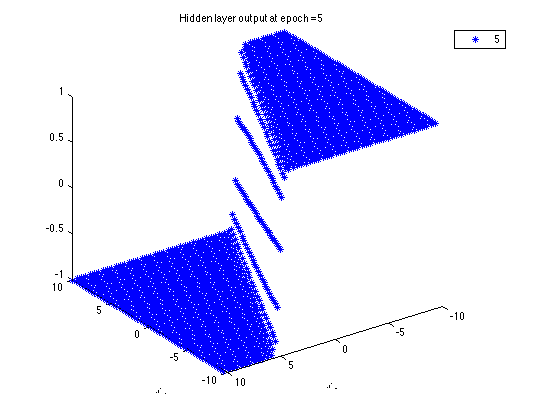
\includegraphics[width=.8\linewidth]{Regression/bivariate/hidden_2layer_5.png}\
  \caption{Epoch 5}
\end{subfigure}%
\begin{subfigure}{.5\textwidth}
  \centering
  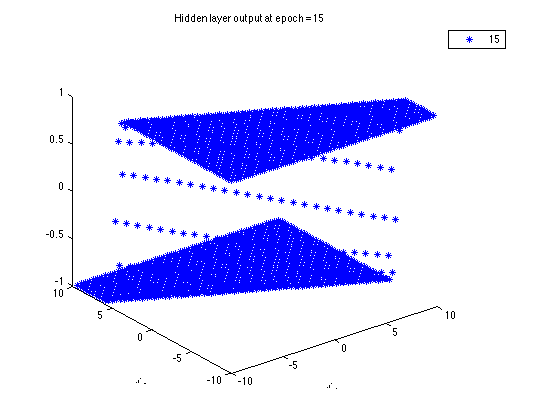
\includegraphics[width=.8\linewidth]{Regression/bivariate/hidden_2layer_15.png}
   \caption{Epoch 15}
  \end{subfigure}
  
  \begin{subfigure}{.5\textwidth}
  \centering
  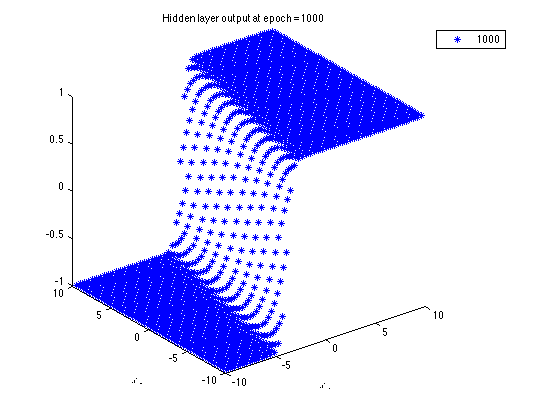
\includegraphics[width=.8\linewidth]{Regression/bivariate/hidden_2layer_1000.png}\
  \caption{End of training}
\end{subfigure}%
  
\caption{Output of output layer node}
\end{figure}

\textbf{Observations :}
\begin{itemize}
\item Both the models of neural networks, i.e. with 1 and 2 hidden layers seemed to perform well in the surface fitting task.
\item The non-linearities in the surface to be approximated are captured by using the tanh sigmoidal function in the hidden layer nodes. 
\item Though very slight overfitting is observed, the models obtained have good generalization ability.  

\end{itemize}
